\scanpage{43}
\mspage{\handwritten{11}}
\uline{11.- Affine group preschemes.}

\uline{\handwritten{11}.0.}- Notation : let $S$ be a prescheme, $X$ an $S$-prescheme, $f:X\handwritten{\to}S$ the structure morphism; we put $\handwritten{\unsure{\mathcal{A}|a}}(X)=f_{\handwritten{*}}(\handwritten{\mathcal{O}}_X)$.

\handwritten{\makebox[0pt][l]{\raisebox{-2ex}{\begin{tikzpicture}[x=1cm,y=1cm]\draw (.05,.14) -- (.05,-.07) -- (.13,-.07);\end{tikzpicture}}}}\uline{Lemma 11.1.- Let $X$ and $Y$ be two $S$-preschemes quasi-compact and quasi-separated over $S$, $f:X\handwritten{\to}S$ and $g:Y\handwritten{\to}S$ the structure morphisms. Then the canonical homomorphism}
\[
\handwritten{\varphi}:\handwritten{\mathcal{A}}(X)\handwritten{\otimes}_{\handwritten{\mathcal{O}}_{\unsure{\mathbb{S}|S}}}\handwritten{\mathcal{A}}(Y)\handwritten{\longrightarrow}\handwritten{\mathcal{A}}(X\handwritten{\times}_S Y)
\]
% Curved pen mark below the tensor-base index.
\figure{\handwritten{\begin{tikzpicture}[x=1cm,y=1cm]\draw (0,.18) .. controls (.25,-.2) and (.8,-.18) .. (1.25,.22);\end{tikzpicture}}}
\margin{\handwritten{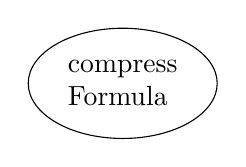
\begin{tikzpicture}[x=1cm,y=1cm]
\draw (0,0) ellipse (1.2 and .7);
\node[align=left] at (0,0) {compress\\Formula};
\end{tikzpicture}}}
\uline{is an isomorphism in each of the following cases :}

\uline{a) $f$ and $g$ are affine}

\uline{b) $f$ or $g$ is flat and affine}

\uline{c) $g$ is flat and $f_{\handwritten{*}}(\handwritten{\mathcal{O}}_X)$ is a flat $\handwritten{\mathcal{O}}_S$-Module.}
% Curved pen mark below the star of f in c).
\figure{\handwritten{\begin{tikzpicture}[x=1cm,y=1cm]\draw (0,.15) .. controls (.15,-.16) and (.45,-.16) .. (.6,.16);\end{tikzpicture}}}
\margin{\handwritten{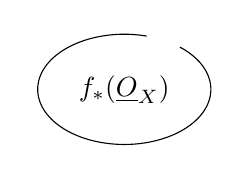
\begin{tikzpicture}[x=1cm,y=1cm]
\draw (.285,.676) arc[start angle=75,end angle=410,x radius=1.1,y radius=.7];
\node at (0,0) {$f_*(\underline{O}_X)$};
\end{tikzpicture}}}

In case b), one may suppose that it is $g$ that is flat and affine. Put $S'=\operatorname{Spec}\handwritten{\mathcal{A}}(X)$ $Y'=Y\handwritten{\times}_S\unsure{\mathbb{S}|S}'$, $g'=g\handwritten{\times}_S S'$ and denote by $v$ the morphism $S'\handwritten{\to}S$. Then $Y$ is quasi-compact and quasi-\linebreak -separated over $S$, and, either $S'$is flat over $S$ (case c) by (EGA III (1.4.15.5)), or $g$ is affine (cases a) and b)). Then (EGA III 1.4.15 and IV 1.2.7 or II 1.5.2), we have :
\[
g'_{\handwritten{*}}(\handwritten{\mathcal{O}}_{Y'})=v^{\handwritten{*}}g_{\handwritten{*}}(\handwritten{\mathcal{O}}_Y)=\handwritten{\mathcal{A}}(Y)\handwritten{\otimes}_{\handwritten{\mathcal{O}}_S}\handwritten{\mathcal{O}}_{S'}.
\]

By (EGA II 1.2.7), $f$ \unsure{factors|factors} through $v$ by means \handwritten{\makebox[0pt][l]{\raisebox{2ex}{\begin{tikzpicture}[x=1cm,y=1cm]\draw (0,0) -- (.17,.09) -- (.43,-.05);\end{tikzpicture}}}}of a morphism $p:G\handwritten{\to}S'$, and we have : $X\handwritten{\times}_S Y=X\handwritten{\times}_{S'}Y'$ and $p_{\handwritten{*}}(\handwritten{\mathcal{O}}_X)=\handwritten{\mathcal{O}}_{S'}$. Since $v$ and $f$ are quasi-compact and quasi-separated,\deleted{over} the same is true of $p$ (EGA IV 1.2.2 and 1.2.4)\handwritten{;} \handwritten{E}ither $Y$ is flat over $S$ (cases b) and c)) and then $Y'$ is flat over $S'$, or $X$ is affine over $S$ (case a)), and then $p$ is an isomorphism. In the first case, we can again apply (EGA III 1.4.15 and IV 1.2.7), and in both cases, we find :
\[
\deleted{\unsure{p_*|q_*}\ \unsure{=}\ \unsure{q'_*|p'_*}}\ p'_{\handwritten{*}}(\handwritten{\mathcal{O}}_{X\handwritten{\times}_S Y})=g'^{\handwritten{*}}p_{\handwritten{*}}(\handwritten{\mathcal{O}}_X)=g'^{\handwritten{*}}(\handwritten{\mathcal{O}}_{S'})=\handwritten{\mathcal{O}}_{Y'}\handwritten{,\ \text{where }p'=p\times_{S'}Y'.}
\]

Hence :
\[
\handwritten{\mathcal{A}}(X\handwritten{\times}_S Y)=v_{\handwritten{*}}g'_{\handwritten{*}}p'_{\handwritten{*}}(\handwritten{\mathcal{O}}_{X\handwritten{\times}_S Y})=v_{\handwritten{*}}g'_{\handwritten{*}}(\handwritten{\mathcal{O}}_{\handwritten{Y}'})=v_{\handwritten{*}}(\handwritten{\mathcal{A}}(Y)\handwritten{\otimes}_{\handwritten{\mathcal{O}}_S}\handwritten{\mathcal{O}}_{S'})=\handwritten{\mathcal{A}}(Y)\handwritten{\otimes}_{\handwritten{\mathcal{O}}_S}\handwritten{\mathcal{A}}(X)
\]
by (EGA II 1.4.7).

\uline{Corollary 11\handwritten{\unsure{.|/}}2.- One defines a functor $X\handwritten{\rightsquigarrow}\operatorname{Spec}\handwritten{\mathcal{A}}(X)$ from the full subcategory of $\operatorname{Sch}_{/S}$ of flat quasi-compact and quasi-separated $X$-preschemes over $S$ such that $\handwritten{\mathcal{A}}(X)$ is a flat $\handwritten{\mathcal{O}}_S$-Module , to that of flat and affine $S$-preschemes over $S$ . This functor commutes with finite products, hence transforms $S$-groups into $S$-groups.}
% archive sheet number: 42
